%compile with pdflatex on papeeria

\documentclass[a4paper,12pt]{article}
\usepackage{fancyhdr}
\usepackage{fancyheadings}
\usepackage[ngerman,german]{babel}
\usepackage{german}
\usepackage[utf8]{inputenc}
%\usepackage[latin1]{inputenc}
\usepackage[active]{srcltx}
%\usepackage{algorithm}
%\usepackage[noend]{algorithmic}
\usepackage{amsmath}
\usepackage{amssymb}
\usepackage{amsthm}
\usepackage{bbm}
\usepackage{enumerate}
\usepackage{graphicx}
\usepackage{ifthen}
\usepackage{listings}
\usepackage{enumitem}
%\usepackage{struktex}
\usepackage{hyperref}


\pagenumbering{gobble}

%%%%%%%%%%%%%%%%%%%%%%%%%%%%%%%%%%%%%%%%%%%%%%%%%%%%%%
%%%%%%%%%%%%%% EDIT THIS PART %%%%%%%%%%%%%%%%%%%%%%%%
%%%%%%%%%%%%%%%%%%%%%%%%%%%%%%%%%%%%%%%%%%%%%%%%%%%%%%
\newcommand{\Fach}{2. Stegreifaufgabe aus der Mathematik (A)}
\newcommand{\Name}{}
\newcommand{\datum}{}
\newcommand{\Matrikelnummer}{}
\newcommand{\Semester}{Q12/1}
\newcommand{\Uebungsblatt}{} %  <-- UPDATE ME
%%%%%%%%%%%%%%%%%%%%%%%%%%%%%%%%%%%%%%%%%%%%%%%%%%%%%%
%%%%%%%%%%%%%%%%%%%%%%%%%%%%%%%%%%%%%%%%%%%%%%%%%%%%%%

\setlength{\parindent}{0em}
\topmargin -1.0cm
\oddsidemargin 0cm
\evensidemargin 0cm
\setlength{\textheight}{9.2in}
\setlength{\textwidth}{6.0in}

%%%%%%%%%%%%%%%
%% Aufgaben-COMMAND
\newcommand{\Aufgabe}[1]{
  {
  \vspace*{0.5cm}
  \textsf{\textbf{Aufgabe #1}}
  \vspace*{0.2cm}
  
  }
}
%%%%%%%%%%%%%%
\hypersetup{
    pdftitle={\Fach{}: Übungsblatt \Uebungsblatt{}},
    pdfauthor={\Name},
    pdfborder={0 0 0}
}

\lstset{ %
language=java,
basicstyle=\footnotesize\tt,
showtabs=false,
tabsize=2,
captionpos=b,
breaklines=true,
extendedchars=true,
showstringspaces=false,
flexiblecolumns=true,
}

\title{Übungsblatt \Uebungsblatt{}}
\author{\Name{}}

\begin{document}
\thispagestyle{fancy}
%\lhead{\sf \large \Fach{} \\ %\small \Name{} - \Matrikelnummer{}
\lhead{\sf \large \Fach{} %\small \Name{} - \Matrikelnummer{}
}
\rhead{\sf \Semester{}   \datum{}}
%\rhead{\sf \Semester{} }
\vspace*{0.2cm}
%\begin{center}
%%\LARGE \sf \textbf{Übungsblatt \Uebungsblatt{}}
%\end{center}
%\vspace*{0.2cm}

%%%%%%%%%%%%%%%%%%%%%%%%%%%%%%%%%%%%%%%%%%%%%%%%%%%%%%
%% Insert your solutions here %%%%%%%%%%%%%%%%%%%%%%%%
%%%%%%%%%%%%%%%%%%%%%%%%%%%%%%%%%%%%%%%%%%%%%%%%%%%%%%

  Name: \underline{\hspace{7cm}}
  \hfill
  Datum: \underline{\hspace{4cm}}

\vspace{1cm}

\Aufgabe{1:}
Berechnen Sie die Integrale:

\begin{enumerate}[label={\alph*)}]
  \item $ \int \frac{x^3-2x^2-5x-7}{3x^2} dx $ 
    \vspace{1cm}
  \item $ \int \frac{4}{\sqrt[4]{-0.25x+4}} dx $
    \vspace{1cm}
  \item $ \int \ln(3x-2) dx $
    \vspace{1cm}
  \item $ \int xe^{-3x^2+2} dx $
    \vspace{1cm}
  \item $ \int \frac{4}{-3x-2} dx $
    \vspace{1cm}
  \item $ \int \frac{3x-2.5}{3x^2-5x+7} dx $
    \vspace{1cm}
  \item $ \int (2tx-e+x^2-t^2) dt $
    \vspace{1cm}
\end{enumerate}

\begin{flushright}7BE \end{flushright}

  \newpage
\Aufgabe{2:}
Gegeben ist der Graph einer Funktion $f$, der mit der $x$-Achse zwei orientierte Teilflächen $A_1$ und $A_2$ einschließt.

\begin{figure}[h!]
  \centering
  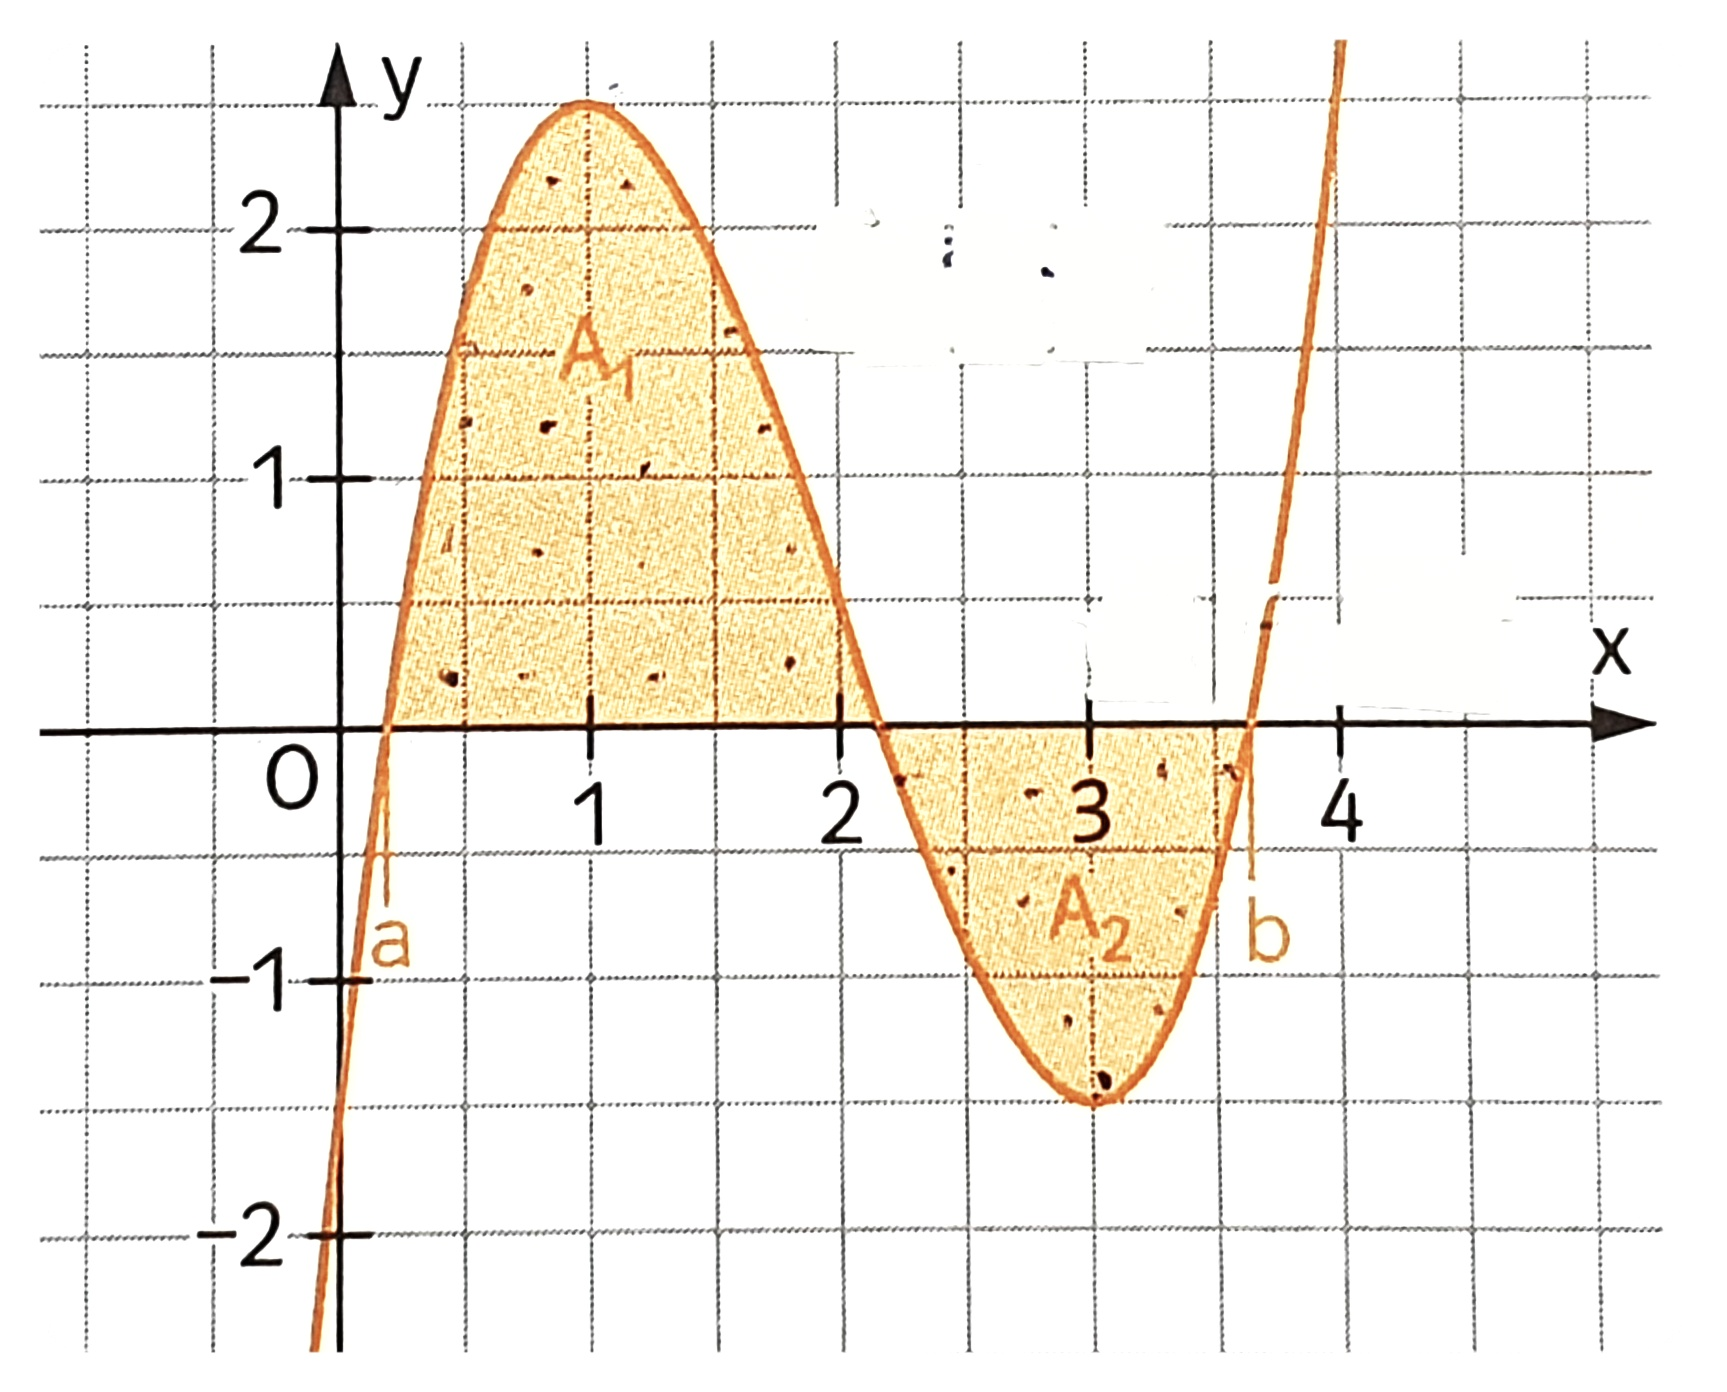
\includegraphics[width=0.5\columnwidth]{Q12_2EX_Integral_1.jpg}
  %\caption{A boat.}
  %\label{fig:boat1}
\end{figure}

\begin{enumerate}[label={\alph*)}]
  \item Das Integral $\int_{a}^{b}f(x)dx=2$. Kreuzen Sie jeweils die richtige Antwort an:\\
    \begin{tabular}{ p{7cm} | p{3cm} | p{3cm} | }
      \cline{2-3}
      %\multicolumn{1}{c}{} & \multicolumn{1}{c}{wahr} & \multicolumn{1}{c}{falsch} \\
        &wahr & falsch \\
      \hline
      \multicolumn{1}{|l|}{$|A_1|$ is doppelt so groß wie $|A_2|$} &  &  \\ \hline
      \multicolumn{1}{|l|}{$|A_1|=|A_2|+2$} & &  \\ \hline
      \multicolumn{1}{|l|}{$|A_1|=2$} & &  \\ \hline
      \multicolumn{1}{|l|}{$A_1>0$ und $A_2<0$} & &  \\ \hline
      \multicolumn{1}{|l|}{$|A_1|$ ist um 2 größer als $|A_2|$} & &  \\ \hline
    \end{tabular}

  \item Bestimmen Sie näherungsweise den Wert des Integrals $\int_{2,2}^{b} f(x)dx$.
  \item Was lässt sich über zwei beliebigen Teilflächen $A_1$ (oberhalb der $x$-Achse) und $A_2$ (unterhalb der $x$-Achse) aussagen, wenn gilt $\int_{b}^{a}f(x)dx=1$ und $a<b$.
\end{enumerate}
\begin{flushright}7BE \end{flushright}


%%%%%%%%%%%%%%%%%%%%%%%%%%%%%%%%%%%%%%%%%%%%%%%%%%%%%%
%%%%%%%%%%%%%%%%%%%%%%%%%%%%%%%%%%%%%%%%%%%%%%%%%%%%%%
\end{document}
